\documentclass[10pt]{article}


\usepackage{latexsym}
\usepackage{amsmath}
\usepackage{amssymb}
\usepackage{amsfonts}
\usepackage{amsthm}
\usepackage{amscd}
\usepackage{epsfig}
\usepackage{verbatim}
\usepackage{fancybox}
\usepackage{moreverb}
\usepackage{graphicx}
\usepackage{psfrag}
\usepackage{hyperref}
\usepackage[all]{xy}
\usepackage[toc,page]{appendix}
\usepackage[subnum]{cases}
\usepackage{bm}
\usepackage{framed}
\usepackage{color}
\usepackage{dsfont}
\usepackage{textcomp}
\usepackage{graphicx}
\usepackage{url}

\textheight 25cm    \textwidth 16cm
\voffset=-4cm
\hoffset=-1.8cm


\title{\fbox{\begin{minipage}{1\textwidth}
\vspace{0,2cm}
\begin{center}
{\huge \textbf{\underline{Report :} Parallel computation of $\pi$ decimals}}
\end{center}
\end{minipage}}}



\author{Alexandre Temperville, Master 2 Scientific Computing}

\date{}



\begin{document}

\maketitle

All that we need to deal with this report is in the folder 'Pi'. 


\section*{The first $\pi$ decimals}


The Leibniz formula gives $\pi$ : $$\pi = 4\, \arctan(1) = 4\,\sum_{k=0}^{+\infty} \cfrac{(-1)^k}{2\,k+1}.$$

Let us define $f$ such that $f(k) = 4\,\cfrac{(-1)^k}{2\,k+1}$.

As $|f(k)| > |f(k + 1)| \;\;\forall k \in \mathbb{N}$, and as this sum is obviously an alternating one, we can claim that it converges towards a real number : $\pi$. This is a well-known result known as the Leibniz test (or in French: "th\'{e}or\`{e}me de convergence des s\'{e}ries altern\'{e}es"). \\

Let us denote
\begin{align*}
S_n \, &= \, 4\,\;\;\sum_{k=0}^{n}\;\; \cfrac{(-1)^k}{2\,k+1} \;\;= \;\;\sum_{k=0}^{n}\;\; f(k) \;\; \mbox{ \textit{and}} \\
R_n \, &= \,4\,\sum_{k=n+1}^{+\infty} \cfrac{(-1)^k}{2\,k+1} \;\;= \sum_{k=n+1}^{+\infty} f(k)
\end{align*}

We have : $$\forall n \in \mathbb{N},\;\; \pi = S_n + R_n.$$

The Leibniz test also states that : $$\forall n \in \mathbb{N}, \;\; |R_n| < |f(n + 1)| \;\; \mbox{ \textit{i.e.} } R_n \mbox{ \textit{is bounded by} } |f(n + 1)|.$$.

We can take $n$ such that $|f(n+1)| < 10^i$, then : $$|R_n| = |S - S_n| < 10^{-i}, \;\; \mbox{ \textit{i.e.} } S_n \in [S - 10^{-i}, S + 10^{-i}].$$ 

Under this condition $S_n$ gives an approximation of $\pi$ with $i-1$ exact decimals. We will use this condition to stop the computation of the sum with a precision of $i$ decimals :
\begin{align*}
\Big(|f(n + 1)| < 10^{-i}\Big) \; &\Longleftrightarrow \; \left(\cfrac{4}{2\,n+3} < 10^{-i}\right) \; \Longleftrightarrow \; \left(\cfrac{4\times 10^i-3}{2} < n\right) \; \Longleftrightarrow \; \left(2\times 10^i -\cfrac{3}{2} < n\right) \\
& \Longleftrightarrow \; \Big(2\times 10^i - 1 \leq n\Big)
\end{align*}
If we compute $S_n$ with $n$ such that the previous inequality is verified, then we will have an exact approximation of $\pi$ up to $i-1$ decimals. \\

\newpage

\; \vspace*{2cm}
\section*{Algorithm in parallel}

This algorithm is also explained in french in the program \textit{pi.c}. \\

To get an approximation of $\pi$ up to $i-1$ decimals, where $i$ is given as a parameter by the user when running the program, we will share out the calculation of the sum between processors, with the number of processors given as a parameter too. \\

We can choose $n = 2\times 10^i - 1$ to satisfy the condition of the previous part. We can see that we need $2\times 10^i$ terms (variable \textit{nb\_termes}) of the sum to reach such precision. $n$ chosen like this allows to find easily a regular split of the sum to do in each processor. As we cannot parallelize the sum asking different processors to compute one decimal for example, we need to separate computations to get each decimals when we have the total sum of the terms. \\

To get $i-1$ exact decimals : if the number of processes is $P$, and if the rank of a process is $rank$, each process will compute a sum of $\cfrac{2\times 10^i}{P}$ terms and stores the result in a variable $partial\_sum$. \\

Finally, we do a reduction with add in process of rank $0$, that will compute the result of $\pi$ with the precision we want thanks to the variable $total\_sum$ and return it on the screen and in a file \textit{pi.dat}.


\section*{Execution of the program}

I tried to test my program on \textbf{g5k} in the frontend of Lille, and we obtain the results described in the picture \textit{\textbf{g5k.png}}. We see with the \textit{ls} command that the results are saved in the file \textit{pi.txt}, I have some warning for \textit{malloc}, I do not understand why.\\

I follow the instructions in the following web-site to work with MPI successfully :

\; \hspace{2cm} \url{http://www.grid5000.fr/mediawiki/index.php/Run_MPI_On_Grid'5000} \\

To do that, on the frontend of Lille, I make a reservation : \textit{oarsub -I -t allow\_classic\_ssh -l nodes=3}. \\
Then, I enter the instructions we can see in the picture \textit{g5k.png}. \\

Here we can see what I obtain in my own computer : \\
\begin{center}
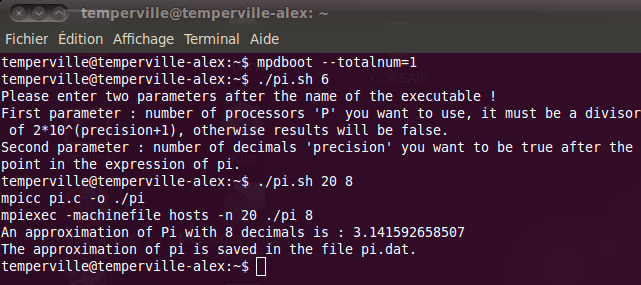
\includegraphics[scale=0.5]{myPC.png} 
\end{center}

On my computer, I run the script \textit{pi.sh} which compiles and the file \textit{pi.c} and runs the executable \textit{pi} with 2 parameters, the first one is the number of processors to use and the second one is the number of decimals we want to be exact. I notice that when I want more than 8 exacts decimals, it is too for my computer (too many computations and precision too high).

\end{document}